% Template for Elsevier CRC journal article
% version 1.2 dated 09 May 2011

% This file (c) 2009-2011 Elsevier Ltd.  Modifications may be freely made,
% provided the edited file is saved under a different name

% This file contains modifications for Nuclear Physics B Proceedings Supplement

% Changes since version 1.1
% - added "procedia" option compliant with ecrc.sty version 1.2a
%   (makes the layout approximately the same as the Word CRC template)
% - added example for generating copyright line in abstract

%-----------------------------------------------------------------------------------

%% This template uses the elsarticle.cls document class and the extension package ecrc.sty
%% For full documentation on usage of elsarticle.cls, consult the documentation "elsdoc.pdf"
%% Further resources available at http://www.elsevier.com/latex

%-----------------------------------------------------------------------------------

%%%%%%%%%%%%%%%%%%%%%%%%%%%%%%%%%%%%%%%%%%%%%%%%%%%%%%%%%%%%%%
%%%%%%%%%%%%%%%%%%%%%%%%%%%%%%%%%%%%%%%%%%%%%%%%%%%%%%%%%%%%%%
%%                                                          %%
%% Important note on usage                                  %%
%% -----------------------                                  %%
%% This file should normally be compiled with PDFLaTeX      %%
%% Using standard LaTeX should work but may produce clashes %%
%%                                                          %%
%%%%%%%%%%%%%%%%%%%%%%%%%%%%%%%%%%%%%%%%%%%%%%%%%%%%%%%%%%%%%%
%%%%%%%%%%%%%%%%%%%%%%%%%%%%%%%%%%%%%%%%%%%%%%%%%%%%%%%%%%%%%%

\documentclass[3p,times,procedia]{elsarticle}

\graphicspath{{fig/}}

\usepackage{nupha_ecrc}
\usepackage{amsmath}

%% The ecrc package defines commands needed for running heads and logos.
%% For running heads, you can set the journal name, the volume, the starting page and the authors

%% set the volume if you know. Otherwise `00'
\volume{00}

%% set the starting page if not 1
\firstpage{1}

%% Give the name of the journal
\journalname{Nuclear Physics A}

%% Give the author list to appear in the running head
%% Example \runauth{C.V. Radhakrishnan et al.}
\runauth{J.S.\ Moreland, J.E.\ Bernhard, W.\ Ke, S.A.\ Bass}

%% The choice of journal logo is determined by the \jid and \jnltitlelogo commands.
%% A user-supplied logo with the name <\jid>logo.pdf will be inserted if present.
%% e.g. if \jid{yspmi} the system will look for a file yspmilogo.pdf
%% Otherwise the content of \jnltitlelogo will be set between horizontal lines as a default logo

%% Give the abbreviation of the Journal.
\jid{nupha}

%% Give a short journal name for the dummy logo (if needed)
\jnltitlelogo{Nuclear Physics A}

%% Hereafter the template follows `elsarticle'.
%% For more details see the existing template files elsarticle-template-harv.tex and elsarticle-template-num.tex.

%% Elsevier CRC generally uses a numbered reference style
%% For this, the conventions of elsarticle-template-num.tex should be followed (included below)
%% If using BibTeX, use the style file elsarticle-num.bst

%% End of ecrc-specific commands
%%%%%%%%%%%%%%%%%%%%%%%%%%%%%%%%%%%%%%%%%%%%%%%%%%%%%%%%%%%%%%%%%%%%%%%%%%

%% The amssymb package provides various useful mathematical symbols
\usepackage{amssymb}
%% The amsthm package provides extended theorem environments
%% \usepackage{amsthm}

%% The lineno packages adds line numbers. Start line numbering with
%% \begin{linenumbers}, end it with \end{linenumbers}. Or switch it on
%% for the whole article with \linenumbers after \end{frontmatter}.
%% \usepackage{lineno}

%% natbib.sty is loaded by default. However, natbib options can be
%% provided with \biboptions{...} command. Following options are
%% valid:

%%   round  -  round parentheses are used (default)
%%   square -  square brackets are used   [option]
%%   curly  -  curly braces are used      {option}
%%   angle  -  angle brackets are used    <option>
%%   semicolon  -  multiple citations separated by semi-colon
%%   colon  - same as semicolon, an earlier confusion
%%   comma  -  separated by comma
%%   numbers-  selects numerical citations
%%   super  -  numerical citations as superscripts
%%   sort   -  sorts multiple citations according to order in ref. list
%%   sort&compress   -  like sort, but also compresses numerical citations
%%   compress - compresses without sorting
%%
%% \biboptions{comma,round}

% \biboptions{}

% macros
\newcommand{\trento}{T\raisebox{-0.3ex}{R}ENTo}
\newcommand{\sig}{\sigma^\mathrm{inel}_{pp}}
\newcommand{\T}{\tilde{T}}
\newcommand{\e}{\varepsilon}
\newcommand{\paddedhline}{\noalign{\smallskip}\hline\noalign{\smallskip}}
\newcommand{\vn}{\sqrt{\langle v_n^2 \rangle}}
\newcommand{\en}{\sqrt{\langle \varepsilon_n^2 \rangle}}

% if you have landscape tables
\usepackage[figuresright]{rotating}

% put your own definitions here:
%   \newcommand{\cZ}{\cal{Z}}
%   \newtheorem{def}{Definition}[section]
%   ...

% add words to TeX's hyphenation exception list
%\hyphenation{author another created financial paper re-commend-ed Post-Script}

% declarations for front matter
\usepackage{graphicx}

\begin{document}

\begin{frontmatter}

%% Title, authors and addresses

%% use the tnoteref command within \title for footnotes;
%% use the tnotetext command for the associated footnote;
%% use the fnref command within \author or \address for footnotes;
%% use the fntext command for the associated footnote;
%% use the corref command within \author for corresponding author footnotes;
%% use the cortext command for the associated footnote;
%% use the ead command for the email address,
%% and the form \ead[url] for the home page:
%%
%% \title{Title\tnoteref{label1}}
%% \tnotetext[label1]{}
%% \author{Name\corref{cor1}\fnref{label2}}
%% \ead{email address}
%% \ead[url]{home page}
%% \fntext[label2]{}
%% \cortext[cor1]{}
%% \address{Address\fnref{label3}}
%% \fntext[label3]{}

%% Instructions from Editor: Please use the following \dochead only in the preprint version (e-print arXiv etc.); 
%% use empty \dochead{} when submitting to Nuclear Physics A!
\dochead{XXVIth International Conference on Ultrarelativistic Nucleus-Nucleus Collisions\\ (Quark Matter 2017)}
%\dochead{}
%% Use \dochead if there is an article header, e.g. \dochead{Short communication}
%% \dochead can also be used to include a conference title, if directed by the editors
%% e.g. \dochead{17th International Conference on Dynamical Processes in Excited States of Solids}

\title{Flow in small and large quark-gluon plasma droplets:\\the role of nucleon substructure}

%% use optional labels to link authors explicitly to addresses:
%% \author[label1,label2]{<author name>}
%% \address[label1]{<address>}
%% \address[label2]{<address>}

\author{}

\address{}

\begin{abstract}
We study the effects of nucleon substructure on bulk observables in proton-lead collisions at the LHC using Bayesian methodology. Substructure is added to the \trento\ parametric initial condition model using Gaussian nucleons with a variable number of Gaussian partons. We vary the number and width of these partons while recovering the desired inelastic proton-proton cross section and ensemble averaged proton density. We then run the model through a large number of minimum bias hydrodynamic simulations and measure the response of final particle production and azimuthal particle correlations to initial state properties. Once these response functions are determined, we calibrate free parameters of the model using established Bayesian methodology. We comment of the implied viability of our partonic model and implications for hydrodynamic behavior in small systems.
\end{abstract}

\begin{keyword}
%% keywords here, in the form: keyword \sep keyword
  Bayesian \sep Flow \sep Initial conditions \sep Quark-gluon plasma \sep Small systems

%% MSC codes here, in the form: \MSC code \sep code
%% or \MSC[2008] code \sep code (2000 is the default)

\end{keyword}

\end{frontmatter}

%%
%% Start line numbering here if you want
%%
% \linenumbers

%% main text
\section{Introduction}
\label{}

Recent measurements of azimuthal particle correlations in small collision systems show striking simularities to flow signatures observed in gold-gold and lead-lead collisions, leading many to question if the origin of small system correlations is hydrodynamic in nature.
A key difficulty in assessing the model-to-data consistency of hydrodynamic models in light-light and light-heavy collisions is theoretical uncertainty in the QGP initial conditions.
In this work, we use established Bayesian methodology to parametrize and constrain the QGP initial conditions in small collision systems in order to infer initial state properties with reduced bias.

\begin{figure}
  \centering
  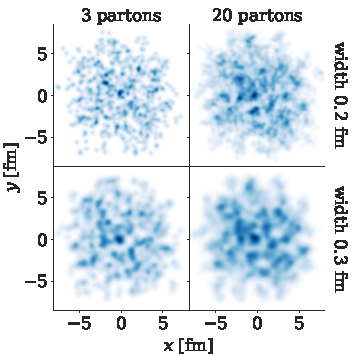
\includegraphics{Pb_thickness} 
  \hspace{8ex}
  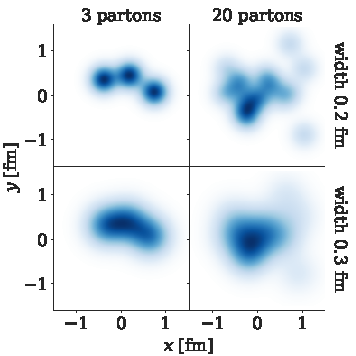
\includegraphics{p_thickness}
  \caption{\label{fig:substructure}
    Nuclear thickness functions $T$ with nucleon substructure for a single lead nucleus (left panel) and proton (right panel) for parton widths $v= 0.2, 0.3$~fm (rows) and parton numbers $m=3,20$ (columns).
  }
\end{figure}

The \trento\ initial condition model used in this work parametrizes local nuclear entropy deposition at midrapidity according to a reduced thickness function
\begin{equation}
  \label{gen_mean}
  \frac{dS}{d^2x\, \tau_0\, d\eta} \bigg\vert_{\eta=0} \propto\, \left(\frac{\T_A^p + \T_B^p}{2}\right)^{1/p}.
\end{equation}
Here $\T$ is the modified participant thickness function $\T(\mathbf{x}) \equiv \sum_{i=1}^{N_\mathrm{part}} \gamma_i\, T_p(\mathbf{x} - \mathbf{x}_i)$, where $\gamma_i$ is a random weight factor sampled from a Gamma distribution with unit mean and fluctuation shape factor $k$, while $T_p$ denotes the proton thickness function described by a normalized Gaussian distribution with nucleon width $w$. 
The exponent $p$ in Eq.~\eqref{gen_mean} is a tunable entropy deposition factor which takes continuous values $p \in (-\infty, \infty)$ and allows the model to mimic various theory calculations. 

Participant nucleons in the colliding nuclei are first determined according to the pairwise collision probability
\begin{equation}
  \label{collision_criteria}
  P_\mathrm{coll}(b) = 1 - \exp[-\sigma_{gg} T_{pp}(b)],
\end{equation}
where $T_{pp}$ denotes the proton-proton overlap function, and the cross section parameter $\sigma_{gg}$ is determined to satisfy the experimentally measured proton-proton cross section $\sig = \int d^2b\, P_\mathrm{coll}(b)$.
The participant nucleons in each nucleus are then used to construct the participant thickness functions $\T_A$ and $\T_B$ which are subsequently passed through the generalized mean in Eq.~\eqref{gen_mean} to furnish the initial transverse entropy density.

%In contrast to alternative initial condition schemes, the model is not derived from effective field theory or based on specific phenomenology. 
%Rather, it is intentionally constructed to maintain maximal flexibility with minimal theoretical assumptions in order to facilitate systematic and unbiased experimental inference.
%Bayesian parameter estimation has correspondingly been used to constrain free parameters of the model concurrently with QGP medium properties.
%These analyses find rather large uncertainties for the preferred nucleon width $w$ and proton-proton fluctuation parameter $k$ with a generalized mean parameter very nearly equal to zero $p \approx 0$.

\section{Nucleon substructure}
\label{}

The generalized mean parameter $p=0$, which optimally describes charged particle yields and flows in heavy nuclei, predicts perfectly Gaussian QGP entropy profiles in high energy proton-proton collisions when the interacting protons are modeled as Gaussians. 
By construction, such profiles will never drive anisotropic transverse flow and hence could not be used to investigate hydrodynamic behavior in small collision systems where the system size approaches the proton length scale.

One possible solution to resolve the apparent conflict is to replace Gaussian protons with deformed or lumpy protons.
In this work, we extend the \trento\ formalism by replacing each Gaussian nucleon with a fixed number of Gaussian partons, described by a variable parton number $N_\mathrm{partons}$ and Gaussian width $v$.
The new proton thickness function $T_p$ thus becomes
\begin{equation}
  T_p(\mathbf{x}) = \gamma_i \sum\limits_{i=1}^{N_\mathrm{partons}} \frac{1}{2 \pi v^2} \exp\left[{-}\frac{(\mathbf{x} - \mathbf{x}_i)^2}{2 v^2}\right],
\end{equation}
where the parton positions $\mathbf{x}_i$ are sampled from the deconvolved radial distribution $r_\mathrm{parton} = \sqrt{w^2 - v^2}$, and $\gamma_i$ is a Gamma random weight factor as before.
Once the nucleon width, parton number, and parton width are specified, we apply Eq.~\eqref{collision_criteria} to each pair of partons and flag each corresponding nucleon as a participant if one or more of its partons collide.
If any parton in a given nucleon participates, \emph{all} partons in that nucleon contribute to the participant thickness function.
Finally, we numerically tune the cross section parameter $\sigma_{gg}$ which now modulates the parton-parton interaction probability in order to recover the desired p+p inelastic cross section.
Figure~\ref{fig:substructure} shows several examples of the nucleon substructure effect on proton and lead nuclear thickness functions.

\section{Model calibration}
\label{}
The aforementioned substructure extension includes a number of free parameters, e.g. the parton number and parton width, which characterize the initial conditions.
These parameters form a complex, multi-dimensional design space which renders manual and brute force optimization methods prohibitively expensive. 
To circumvent this issue, we apply established Bayesian methodology and use Monte Carlo methods to sample the posterior distribution of the model parameters, calibrated to fit p+Pb collision data at $\sqrt{s}_\mathrm{NN} = 5.02$~TeV measured by the ALICE experiment.
This procedure, described at length in references \ref{}, is briefly summarized as follows.

We first sample $300$ unique parameter configurations using a space filling algorithm to construct a scaffolding of the design space, such that each parameter is sampled from a uniform distribution in a finite range.
The parton width cannot be larger than the nucleon width and hence requires special attention.
We re-parametrize it using a structure parameter
\begin{equation}
  \chi = v_\mathrm{min} + \chi\, (v_\mathrm{max} - v_\mathrm{min}), 
\end{equation}
where the minimum parton width $v_\mathrm{min}=\sqrt{A_\mathrm{min}/N_\mathrm{parton}}$ with $A_\mathrm{min}=0.09 ~\mathrm{fm}^2$ is chosen to always permit a configuration which satisfies the inelastic p+p cross section, and the maximum allowable parton width is capped at $v_\mathrm{max} = w$.
The ranges of the model parameters are shown in Tbl.~\ref{ranges}.
\begin{table}[h]
  \centering
  \begin{tabular}{lll}
    Parameter & Description & Range \\
    \paddedhline
    $p$    & Entropy deposition parameter & $-1$ to $+1$ \\
    $\sigma_\mathrm{fluct}$ & nucleon fluctuation std dev & 0--2 \\
    $\log_2(N_\mathrm{parton}$) & Parton number (log space) & 0--4.5 \\
    $w$    & Nucleon width & 0.4--1 fm \\
    $\chi$ & Nucleon structure & 0--1
  \end{tabular}
  \caption{
    \label{ranges}
  }
\end{table}

We run the \trento\ initial condition model with partonic substructure and calculate the initial entropy density $s$ and eccentricity harmonics $\e_2$ and $\e_3$ for a large number of minimum bias events using the parameter values at each design point.
A Gaussian process emulator is then trained to interpolate these quantities as a function of the parameter values in Tbl.~\ref{ranges}.
The trained emulator admits essentially instant predictions for the entropy density  and eccentricity harmonics in a given centrality bin at arbitrary points in parameter space.

To make contact between initial state properties and final state observables, we generate a large sample of p+Pb initial condition events using randomly sampled substructure parameters and evolve them through event-by-event hybrid model calculations which couple boost-invariant viscous hydrodynamics to a hadronic afterburner.
We then measure the yield and flow response functions 
\begin{align}
  N_\mathrm{ch}(|\eta| < 1) = f(dS/dy), \\
  \frac{\vn}{\en} = g\left(\frac{N_\mathrm{ch}(|\eta| < 1)}{A_0}\right),
\end{align}
where $A_0$ is the transverse area of the entropy profile, measured by counting the cells above 1\% of the peak entropy density. 
The response functions $f$ and $g$ are finally interpolated with a set of basis splines and used to translate the predictions of the Gaussian process emulator from initial state properties to final state observables. 

Finally, the model is calibrated using the Gaussian process emulator and response functions to perform random walks through the parameter space, weighted by the Bayesian posterior probability that the model predictions describe the ALICE data; we calibrate to both the charged particle yields $N_\mathrm{ch}(|\eta| < 1)$ and flow cumulants $v_n\{2\}$ in several centrality bins.
By using a large number of walkers and a large number of steps, we are able to generate a histogram of the walker occupancy density in the multidimensional parameter space.
The resulting posterior distribution is visualized in Fig.~\ref{fig:posterior} which shows projections of the posterior distribution along each model parameter.

\begin{figure}
  \centering
  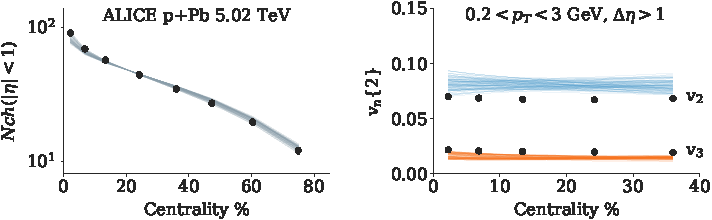
\includegraphics{observables_samples}
  \caption{
    \label{fig:observables} Emulator predictions of 100 random samples drawn from posterior distribution compared to experimental data from the ALICE experiment for p+Pb collisions at $\sqrt{s_\mathrm{NN}} = 5.02$~TeV.
    Left column: charged particle yield $N_\mathrm{ch}(|\eta| < 1)$; right column: two-particle cumulant $v_n\{2\}$ for $0.2 < p_T < 3.0$~GeV and $\Delta \eta > 1$.
  }
\end{figure}

\begin{figure}
  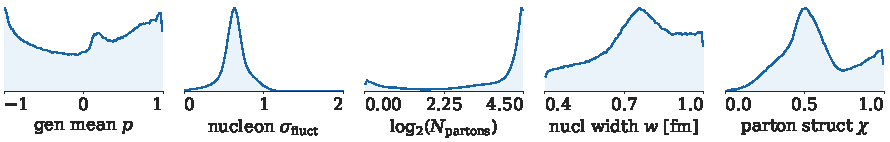
\includegraphics{posterior}
  \caption{
    \label{fig:posterior} Marginalized posterior distributions for the calibrated model.
    Parameters listed from left to right: generalized mean parameter $p$, nucleon fluctuation standard deviation $\sigma_\mathrm{fluct}$, parton number $\log_2(N_\mathrm{partons})$, nucleon width $w$, and parton structure parameter $\chi$.
    Prior distributions were uniform (flat).
  }
\end{figure}


\section{Summary}
\label{}

%% References
%%
%% Following citation commands can be used in the body text:
%% Usage of \cite is as follows:
%%   \cite{key}         ==>>  [#]
%%   \cite[chap. 2]{key} ==>> [#, chap. 2]
%%

%% References with BibTeX database:

\bibliographystyle{elsarticle-num}
\bibliography{<your-bib-database>}

%% Authors are advised to use a BibTeX database file for their reference list.
%% The provided style file elsarticle-num.bst formats references in the required Procedia style

%% For references without a BibTeX database:

% \begin{thebibliography}{00}

%% \bibitem must have the following form:
%%   \bibitem{key}...
%%

% \bibitem{}

% \end{thebibliography}

\end{document}

%%
%% End of file `nupha-template.tex'.
